\section{Multiple Spines}\label{section:multi_spine}

In the previous sections we showed how \PQ-trees relate
to book embeddings. On the one hand they can help to solve
the problem for connected graphs on the pages and on the other hand
we can restrict the orders of the vertices with a \PQ-tree, yielding
an interesting modification to book embedding.

\begin{figure}[\placement]\centering
    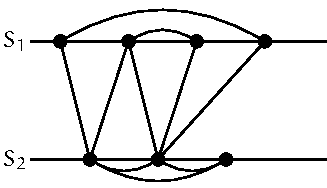
\includegraphics{figures/t_two_spines}
    \caption[Two-spine drawing]{A two-spine drawing.}
    \label{figure:two_spines}
\end{figure}

We now consider another variation on book embedding which 
will turn out to be a special case of the latter application of \PQ-trees.
It is a generalisation of the 2-page case that uses not just one spine but several parallel
spines~(lines) $S_1$, \dots, $S_k$. In the following considerations we always assume
that $S_i$~is above~$S_{i+1}$ for all $i\in\range{k-1}$.
We want to planarly draw one graph above~$S_1$,
one between~$S_i$ and $S_{i+1}$ for each $i \in \range{k-1}$ and one
below~$S_k$, as depicted in \myref{figure:two_spines} for
two spines. This problem is motivated by \emph{level planarity} which
is the same problem without the \emph{caps}, the graph above~$S_1$ and
the graph below~$S_k$.
The level planarity problem was first introduced by Tomii~et.~al.~\cite{Tomii77}. 
Jünger, Leipert and
Mutzel presented an algorithm that checks for level planarity in linear time~\cite{Junger99}.

In this section we show that the multiple spine problem is equivalent to a 2-page book embedding problem constrained by a special \PT-tree, but do not manage to give an efficient algorithm
it. Still, this reinforces our belief that \probPTree is an interesting problem.

Let the spines always be~$S_i = \SR \times \{-i\}$. We now formally define
the problem. It will turn out to be convenient to formally use directed edges pointing downward for the edges between the spines, but we still understand and draw these edges as undirected edges.

\newProb{\probMul}{Vertex sets~$V_1$, \dots, $V_k$ and
edge sets $E_0 \subseteq \binom{V_1}{2}$, $E_1 \subseteq V_1\times V_2$,
\dots, $E_{k-1} \subseteq V_{k-1} \times V_k$, $E_k \subseteq \binom{V_k}{2}$.}{Is there
a planar drawing of $(V_1 \cup \dotsb \cup V_k, E_0 \cup \dotsb \cup E_k)$ such that
a vertex in~$V_i$ lies on~$S_i$ for all~$i \in \range{k}$, edges do not cross a spine,
the edges in~$E_0$ lie completely above~$S_1$ and the edges in~$E_k$ lie completely below~$S_k$?}

Tomii~et.~al.~\cite{Tomii77} showed that the 2-level planar graphs are exactly the forests
of caterpillars. Recall that a \emph{caterpillar} is a tree all of whose vertices are on
a central path or one edge away from it. Therefore, each of the graphs~$(V_i \cup V_{i+1}, E_i)$ for~$i \in \range{k-1}$ has to be a forest, \ie we find~$|E_i| = |V_i| + |V_{i+1}| - l$ if this
forest has $l$~components. That is, as in the case of page embedding the number of edges is again linear in
the number of vertices. Thus, the size of a \probMul~instance is in~$\OO\bigl(|V_1| + \dotsb + |V_k|\bigr)$.

\begin{figure}[\placement]\centering
    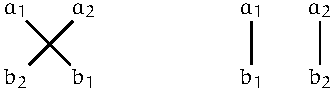
\includegraphics{figures/t_level_order}
    \caption[Level planarity is an ordering problem]{Level planarity only depends on the order of the vertices.}
    \label{figure:level_order}
\end{figure}

From \myref{lemma:constraints} we know that book embedding is essentially an ordering problem.
Similarly, consider two edges $(a_1, b_1)$ and~$(a_2, b_2)$ lying between the same two spines
and investigate how their embeddability depends on the order of their endpoints. If
$a_1$~lies left of~$a_2$ on the upper spine and $b_2$~lies left of~$b_1$ on the lower spine, then any Jordan curve from $a_1$ to~$b_1$ between the spines must intersect with any Jordan curve from $a_2$ to~$b_2$ between the spines by the Jordan curve theorem, \ie there cannot 
be a level embedding with this order. This case is depicted in \myref{figure:level_order}. Similarly,
if $a_2$~lies left of~$a_1$ and $b_1$~lies left of~$b_2$, the edges~$(a_1, b_1)$ and~$(a_2, b_2)$ also
cannot be embedded.

In any other order we can just draw a straight line for both
edges to obtain a valid embedding of the edges. After combining these observations for all pairs
of edges and taking the caps into account, we get a total order formulation of \probMul.
 
\begin{lemma}\label{lemma:multi_spine_total}
Let~$I := (V_1, \dotsc, V_k, E_0, \dotsc, E_k)$ be a \probMul instance. Then~$I$ is solvable
if any only if there is a linear order~$<_i$ on~$V_i$ for each $i \in \range{k}$ such
that the following properties hold. For all~$i \in \{1, \dots, k-1\}$ and pairs of edges~$(a_1, b_1), (a_2, b_2) \in E_i$ the order $a_1 <_i a_2 \land b_2 <_{i+1} b_1$ does not occur. Furthermore,
for $i\in\{0, k\}$ and all $\{a, b\}, \{c, d\} \in E_i$ we must not have $a <_i c <_i b <_i d$.
\end{lemma}

The order constraint for level planarity looks very similar to the book constraint,
just separated into two total orders. Indeed, if we have a \probMul instance we can find a corresponding
book embedding instance.
\begin{figure}\centering
    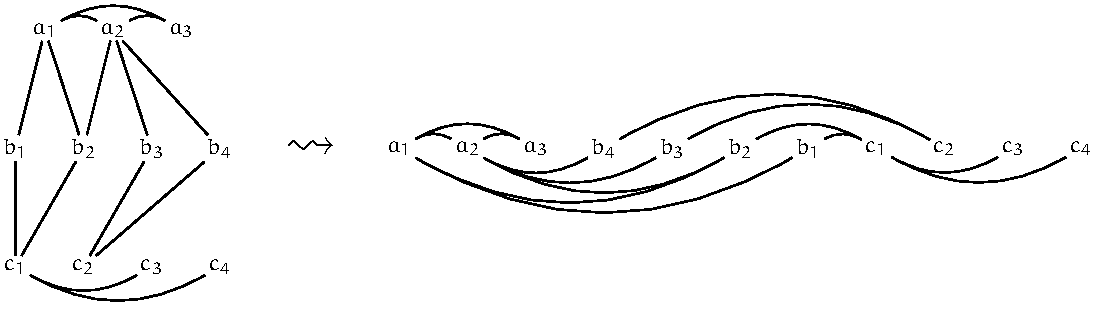
\includegraphics[width=0.9\textwidth]{figures/t_level_map}
    \caption[\probMul instance to book embedding instance]{A \probMul instance can be transformed into a 2-page book embedding instance
with separated sets of vertices.}
    \label{figure:level_map}
\end{figure}
\vskip1em
\begin{theorem}
Let~$I := (V_1, \dotsc, V_k, E_0, \dotsc, E_k)$ be a \probMul instance. We define
a corresponding 2-page book embedding instance by taking $V := V_1 \cup \dotsb \cup V_k$
as vertices and 
\begin{align*}
\widetilde{E}_1 := \bigcup_{\substack{i \in \{0, \dotsc, k\}\\ i \text{\emph{ even}}}} E_i\\
\widetilde{E}_2 := \bigcup_{\substack{i \in \{0, \dotsc, k\}\\ i \text{\emph{ odd}}}} E_i
\end{align*}
as pages. Then~$I$ is solvable if and only if~$J := (V, \widetilde{E}_1, \widetilde{E}_2)$
has a book embedding where the vertices in each~$V_i$ are consecutive.
\end{theorem}

\begin{myproof}
\begin{itemize}
\item[]
\item[``$\Rightarrow$''] Let~$<_i$ for~$i \in \range{k}$ be total orders forming a valid 
embedding of~$I$. 

Then define~$<$ on~$V$ to be the total order that first lists the
vertices of~$V_1$, then the vertices of~$V_2$, and so on. Get the inner order of the vertices
in~$V_i$ from~$<_i$ if~$i$ is even and from~$<_i$ reversed if~$i$ is odd. This
construction is illustrated in \myref{figure:level_map}.

The order~$<$ is a valid solution of the book embedding problem~$J$:
The edges in distinct edge sets~$E_i$ do not intersect by the construction of~$<$ and the definitions
of $\widetilde{E}_1$ and $\widetilde{E}_2$. Edges in~$E_0$ or~$E_k$ do not intersect since~$<_1$
and~$<_k$ are valid page embeddings for~$(V_1, E_0)$ and~$(V_k, E_k)$, respectively. Now take
two edges~$(a_1, b_1), (a_2, b_2) \in E_i$ for some~$i \in \range{k-1}$. If~$a_1 < a_2 < b_1 < b_2$
occurs, we have~$a_1 <_i a_2\;\land\;b_1 <_{i+1} b_2$, contradicting the validity of
the initial solution of~$I$. Thus, the book constraint for the two edges is fulfilled.
\item[``$\Leftarrow$''] Let~$<$ be a valid book order of~$J$ where
the sets~$V_i$ with~$i \in \range{k}$ are separated. Do the construction above in reverse, \ie
define~$<_i$ to be the restriction of~$<$ to~$V_i$ for all~$i \in \range{k}$. Additionally,
reverse~$<_i$ when~$i$ is odd.

The order~$<_i$ yields a valid embedding for~$I$: The caps already appeared in the book embedding
problem~$J$, \ie they are still valid. If~$a_1 <_i a_2\;\land\;b_2 <_{i+1} b_1$ occurs for some~$(a_1, b_1), (a_2, b_2) \in E_i$ and~$i \in \range{k-1}$, then we must have either~$a_1 < a_2 < b_1 < b_2$,
$a_2 < a_1 < b_2 < b_1$, $b_1 < b_2 < a_2 < a_1$ or~$b_2 < b_1 < a_1 < a_2$. All of these
cases contradict the book constraints.\qedhere
\end{itemize}
\end{myproof}

\paragraph{Outlook}

All in all, we see that \probMul is equivalent to a 2-page book
embedding problem where the vertex sets~$V_i$ with~$i \in \range{k}$ have to be 
separated. This separation can be modelled by a \PT-tree by introducing a \PT-node
connected to the vertices~$V_i$ for all~$i \in \range{k}$ and connecting all 
of these \PT-nodes to a single root. 

Since \probMul is an interesting problem in its own right, this leaves several
distinct possibilities for further results:
\begin{itemize}
\item Provide a polynomial time algorithm for  \probPTree and get an efficient solution of \probMul.
\item Prove the \NP-completeness of \probMul and get the \NP-completeness of \probPTree.
\item Provide a polynomial time algorithm for \probMul and get an efficient algorithm for a special case of \probPTree.
\end{itemize}